%%%%%%%%%%%%%
%% METHODS %%
%%%%%%%%%%%%%

%This chapter describes in detail the methods for whatever activities were necessary for your project – e.g., data gathering, data analysis, requirements analysis, design, implementation, testing/evaluation, etc. Your choice of methods should be discussed and justified in view of the project objectives, and with reference to the pertinent literature. Report not only what methods you applied in generic terms, but what you actually did: sufficient information about dates and details for your reader to understand how you ran your project, rather than just how one could run any similar project. 

\chapter{Methods}
\label{Methods} 

This chapter describes the methods used to generate the prediction model.

%-----------------------------------
%	AUTOENCODERS
%-----------------------------------

\section{Autoencoders}

% maybe best moved conda, ros, unity, etc (i.e. plumbing) to appendix, and keep here only the specific network architectures, cameras and camera libraries.

\section{conda}

% https://docs.conda.io/projects/conda/en/latest/index.html

conda (\cite{Conda2021}) is a system that simplifies package management and deployment. It is part of the Anaconda Python distribution. conda allows environments to be created, saved and switched from one to another, such that separate environments can be configured and run. A list of conda commands used in this project is given in \ref{app_methods:conda}. While conda can act as a package installer, it is only used here as an environment manager, while pip is used a a package manager.

\section{pip}

pip (\cite{pip2021}) is a package installer for Python that can be used to install packages from PyPI (the Python Package Index), a repository for the Python programming language, used to distribute software written in Python.

\section{UR3}
% https://www.universal-robots.com/products/ur3-robot/

The original experiment used a UR3 robotic arm
% Tinker Braccio - max load 150g
% https://store.arduino.cc/tinkerkit-braccio-robot
% will probably have to go with that plus a wall mount scenario
% https://www.zivid.com/zivid-one-plus
% SDKs
% https://www.zivid.com/downloads

%%%%%%%%%%%%%%%
% SETUP
%%%%%%%%%%%%%%%
% Hardware
% 1. Zivid One+ camera in fixed position
% 2. Robotic Arm TBA
% 3. Transparent, translucent and opaque object

% Software
% 1. Tensorflow/Keras
% 2. ROS
% 3. Unity

% Models
% 1. Trained network for object detection
% 2. Trained network for path planning / object grasping
% 3. Trained network for command speech recognition - NTH

% All image and path planning data to be generated by Unity
% All audio data to be generated by GAN-like architectures, from a few audio samples

\section{Zivid One+}

\section{Niryo One}
% Train end-to-end to pick-and-place ? :D

% The story we are trying to tell
% 1. We'll retrieve an image RBD + RGBD from camera
% 2. The image x2 goes through a pipeline where the output is a prediction of the 3D space and objects present
% 3. A voice issues a command like move object from A to B
% 4. The 3D space and command are fed to another pipeline, which outputs a path
% the robotic arm needs to follow to move an object from location A to location B
\section{ROS}

\section{ROS x Arduino}

% https://maker.pro/arduino/tutorial/how-to-use-arduino-with-robot-operating-system-ros

% http://wiki.ros.org/rosserial_arduino/Tutorials

\section{Unity}
% Robotics' simulation in Unity
% https://resources.unity.com/unitenow/onlinesessions/simulating-robots-with-ros-and-unity

% Niryo One Robotic Arm in Unity
% https://blogs.unity3d.com/2020/11/19/robotics-simulation-in-unity-is-as-easy-as-1-2-3/

% ROS#
% https://github.com/siemens/ros-sharp

\section{Network Architectures}

In this section we discuss the network architectures used by ClearGrasp and Depth2Depth.



\section{Depth Cameras}

\begin{verbatim}
Start here: https://www.intelrealsense.com/beginners-guide-to-depth/
and take it from there.
Maybe also have a look here:
https://ulir.ul.ie/bitstream/handle/10344/7592/Sivcev_2018_Smart.pdf?sequence=5
Point GrayBumblebee 2 stereo camera
Point Gray BlackFly monocular camera
\end{verbatim}


\section{Prediction Workflow}

\begin{verbatim}
1. Input
2. Networks

eval_depth_completion.py, line 169:

We get the "corrected" output depth likesuch:

output_depth, filtered_output_depth = depthcomplete.depth_completion(
(...)

depth_completion is a method of the DepthToDepthCompletion class,
defined in:

depth_completion_api.py, line 732:
    def depth_completion(self,
    (...)
    which returns numpy arrays:
    
        return self.output_depth, self.filtered_output_depth

Note, these are to compute error metrics, the actual images
are stored during the inference process.

To obtain the two arrays:    
    # perform object segmentation
    def _modify_depth_delete_masks(

 571       self.mask_predicted = self.inferenceMasks.runOnNumpyImage
 
 
 _complete_depth
 
 # SURFACE NORMALS
 (...) self.inferenceNormals.runOnNumpyImage(input_image)
 
 Then, perform boundary detection:
 # OUTLINES
        self.occlusion_weight, self.occlusion_weight_rgb, self.outlines_rgb = self.inferenceOutlines.runOnNumpyImage(
            input_image)
            
            
 
 self.InferenceMasks
 
 3 models
 inference_models.InferenceNormals
 inference_models.InferenceOutlines(
 inference_models.InferenceMasks(
 
In inference_models.py:
 
self.model = deeplab_masks.DeepLab(num_classes=3, backbone='resnet', sync_bn=True,
                            freeze_bn=False)
                            
we get deeplab_masks from

from .modeling import deeplab, deeplab_masks

Network architectures used by each task (normal estimation, boundary detection and 
transparent object segmentation).

InferenceOutlines -> deeplab_resnet

InferenceNormals -> deeplab_resnet

InferenceMasks -> drn

In all three cases, image is presented as an one-dimensional array.
(...)
# Create Transforms
        self.transform = iaa.Sequential([
(...)


\end{verbatim}

\section{OpenEXR}
\begin{verbatim}
https://www.openexr.com/index.html - need a citation

https://scholar.google.com/scholar?hl=en&as_sdt=0%2C5&q=openexr+image+file+format&btnG=&oq=openexr
\end{verbatim}

OpenEXR is not playing well with windows. TODO Try on Ubuntu. Works ok on Ubuntu.

\section{deep2depth}
% from https://arxiv.org/pdf/1803.09326.pdf
"Overall,  our  main  algorithmic  insight  is  that  it  is  bestto  decompose  RGB-D  depth  completion  into  two  stages:1) prediction of surface normals and occlusion boundariesonly from color, and 2) optimization of global surface struc-ture from those predictions with soft constraints providedby observed depths.  During experiments we find with thisproposed  approach  has  significantly  smaller  relative  errorthan alternative approaches. It has the extra benefit that thetrained network is independent of the observed depths andso does not need to be retrained for new depth sensors."  
The one we are interested in are autoenconders and GAN architectures (citations 70 and 58, respectively).


%%%%%%%%%%%%%%%%%%%%%%%%%%%%%%%%%%%%%%%%%%%%%%%%%%%%%%%%%%%%%%%%%
% ClearGrasp Live demo with RealSense 415
%%%%%%%%%%%%%%%%%%%%%%%%%%%%%%%%%%%%%%%%%%%%%%%%%%%%%%%%%%%%%%%%%

% Points to be made
% 1. in realsense.cpp, what is happening in greater detail, how are rgb and depth 
% images being extracted, what are the libraries ?
% 2. What is the format of rgb and depth at that point ?

A pipe object is ini

% realsense camera firmware version 5.12.13.50 upgraded from 05.12.11.00
% camera viewer
% $ realsense-viewer


\section{RealSense 415 ClearGrasp live demo}
% Cleargrasp's realsense.cpp, used to stream images via TCP from camera to prediction engine:
% https://github.com/dsikar/cleargrasp/blob/master/live_demo/realsense/realsense.cpp
% builds on:
% https://github.com/andyzeng/visual-pushing-grasping/blob/master/realsense/realsense.cpp
% The latter was in reinforcement learning to train robotic arms for grasping
ClearGrasp provides source code for a live demo using the Intel RealSense D415 depth camera. Once compiled to ./cleargrasp/live\_demo/build/realsense, the executable can start the camera, which sends image data through TCP port 50010. The image data is displayed on an OpenGL screen (\ref{fig:realsenseOutputForReport}).
\begin{figure}[h!]
\centering
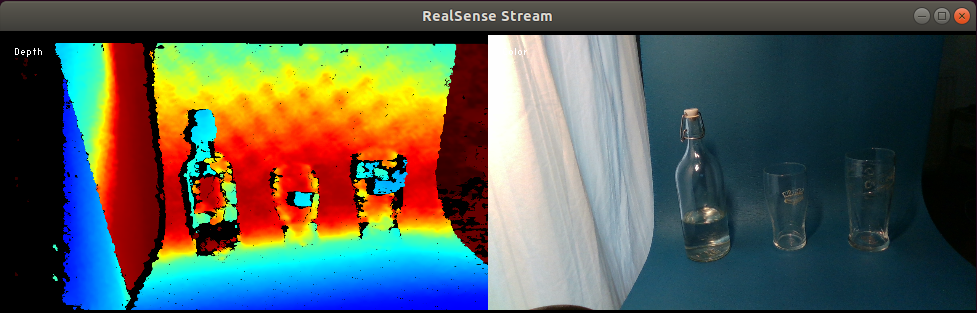
\includegraphics[width=\textwidth]{Figures/realsenseOutputForReport.png}
\caption{RealSense Stream, showing left to right the colourised RGBD and the RGB images}
\label{fig:realsenseOutputForReport}
\end{figure}
The live\_demo.py script loads the configurations defined in config/config.yaml e.g. storage location, weight files (checkpoints) for surface normals, outlines and mask segmentation models, the path to depth2depth executable and so forth. The depth completion API is initialised and the RGB image and input depth obtained from the camera:
\begin{verbatim}
color_img, input_depth = rcamera.get_data()
input_depth = input_depth.astype(np.float32)
\end{verbatim}
rcamera being an object of the realsense library. color\_img is a numpy array of size 720 * 1280 * 3 and of data type 8 bit unsigned integer, input\_depth is a numpy array of size 720 * 1280 and, once type converted, of data type 32 bit float (float32).
\begin{figure}[h!]
\centering
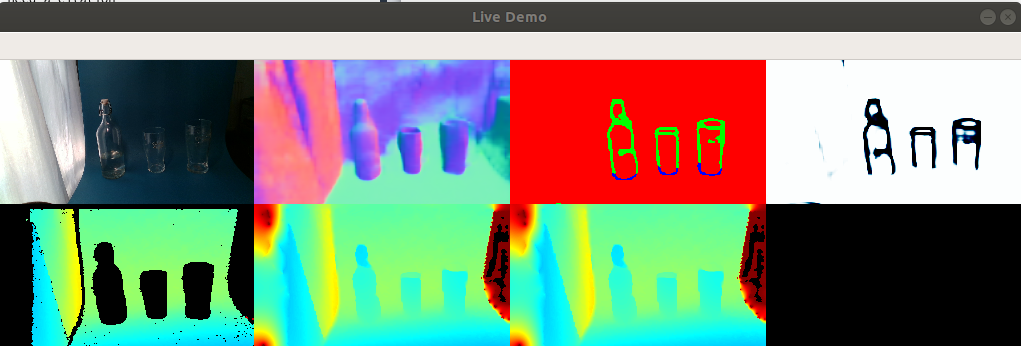
\includegraphics[width=\textwidth]{Figures/ClearGraspLiveDemoForReport.png}
\caption{ClearGrasp live demo, showing on top row, left to right, input RGB image, predicted surface normals, predicted outlines (boundaries) and occlusion boundary weights. Bottom row, left to right, input depth mapped,, output depth mapped, filtered output depth mapped and a blank image to make up the row}
\label{fig:ClearGraspLiveDemoForReport}
\end{figure}

This is the point where the script may be modified to use Zivid One+ data. Figure \ref{fig:ClearGraspLiveDemoForReport} shows the input image, processed outputs and predictions. 

\section{Zivid Studio}
Zivid Studio is a desktop application that enables manual and assisted captures of high-definition point clouds
TODO add citation

\begin{figure}[h!]
\centering
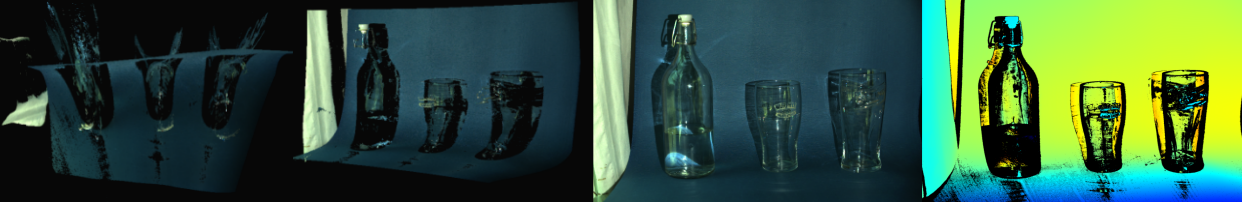
\includegraphics[width=\textwidth]{Figures/ZividStudio.png}
\caption{Zivid Studio captures}
\label{fig:ZividStudio}
\end{figure}

\section{Depth cameras}
Discussion and comparison of Zivid One+ and RealSense 415

\section{Capturing RBG and Depth with the D415}

% The story we want to tell: We want to do some qualitative analysis on the input depth supplied by camera and the one predicted by network.
% To do this, we will visualise two point clouds, one of the RBG plus original depth, and the other of the RBG plus predicted depth.
% Ideally we should also have some metric of noise/cleanliness possibly iterating over every point in the cloud, computing distance to nearest neighbour and deciding on a threshold that would indicate the presence of outliers, which it turn would indicate presence of noise.


\section{Capturing RBG and Depth with the Zivid One+}











